\clearpage
\twocolumn[{%
\subsection{SNR as a surrogate for decision accuracy}
\label{app:rq04_surrogates}

\noindent\begin{minipage}[t]{0.485\textwidth}
\vspace{0pt}
\paragraph{Research Question.} \emph{Before training the reference, can a statistic computed on the proxy alone tell us that the proxy's decision will match the reference's? First among the 22 SNR definitions of the noise-and-SNR analysis: which best correlates with \textbf{decision accuracy} across the ladder's languages, and does the answer survive a change of training seed?}

\paragraph{Setup.} Seed-1904 runs of every cell, 90M--1.7B, on the tasks above chance. For each of 22 SNR definitions, we compute the Pearson $r$ between $\log_{10}$ SNR and decision accuracy over the tasks of one language. We keep the languages with at least three tasks and average over the 50 trained languages. We do this for DA-size (proxy final against 1.7B final) and for DA-ckpt (the early checkpoints of a proxy against its final checkpoint).
\end{minipage}\hfill
\begin{minipage}[t]{0.485\textwidth}
\vspace{0pt}
\begin{rqfinding}
\textbf{1. The relative-spread SNR definitions track decision accuracy best, as a block.} \texttt{rel\_std}, \texttt{rel\_mpd} and \texttt{rel\_dispersion} read mean r 0.54--0.56 with DA-size and 0.57--0.58 with DA-ckpt (0.56--0.57 overall), ahead of \texttt{iqr} (0.53) and the eight dispersion and robust definitions (\texttt{aad}, \texttt{rms\_deviation}, \texttt{dist\_std}, \texttt{mpd}, \texttt{range}, \texttt{dispersion}, \texttt{quartile\_deviation}, \texttt{mad}: 0.49--0.51 overall). The figure's all-task panels read 0.50--0.62 and 0.59--0.64 for their top six, both led by \texttt{rel\_mpd}. The leader \texttt{rel\_std} (0.56 / 0.58) wins by less than 0.01, and the depth definitions are null or anti-signals (\texttt{tukey} $-$0.01 / $-$0.11, \texttt{projection} $-$0.06 / $-$0.14). (Figure~\ref{fig:app_rq04_surrogates}.)
\\
\\
\textbf{2. No exact definition is best everywhere.} Per language the winner is one of 11 definitions under DA-size and one of 12 under DA-ckpt.
\\
\\
\textbf{3. The seed holdout agrees under both DA kinds, on one or two languages.} The global ranking of the 22 definitions correlates across the seed split at Spearman $\rho$ 0.70 under DA-ckpt and 0.55 under DA-size.
\end{rqfinding}
\end{minipage}

\vspace{\baselineskip}
\noindent\begin{minipage}{\textwidth}
\centering
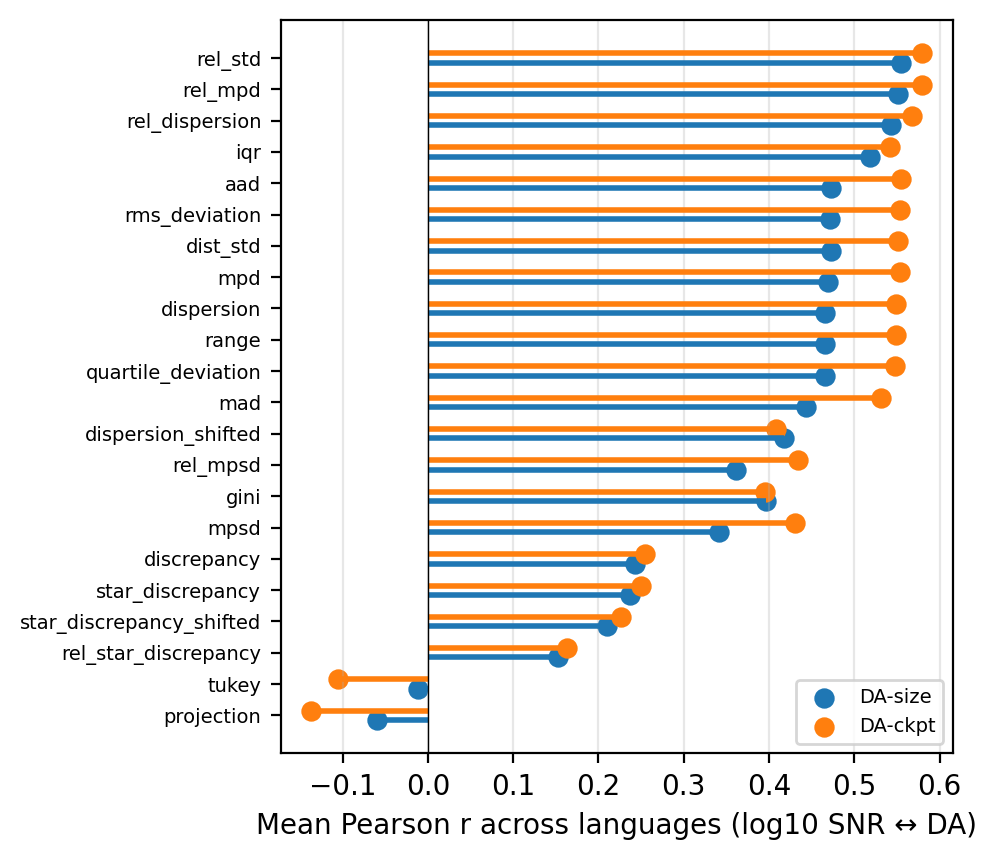
\includegraphics[width=\textwidth,height=0.36\textheight,keepaspectratio]{figures/app_rq04_surrogates.png}
% source: src/signal-and-noise/analysis/rq04_surrogates/pretraining/predictivity/top_variants_overall_paper.png
\captionof{figure}{\textbf{The relative-spread SNR definitions track decision accuracy best, as a block.} For each of the 22 SNR definitions, the mean over languages of the Pearson r between log$_{10}$ SNR and decision accuracy across the tasks of one language, for DA-size (blue) and DA-ckpt (orange). The definitions are ordered by their DA-size correlation.}
\label{fig:app_rq04_surrogates}
\end{minipage}
\vspace{\baselineskip}
}]
